\documentclass[a4paper, 10pt]{article}
\usepackage{../../CEDT-Homework-style}

\usepackage{amsmath}
\allowdisplaybreaks

\setlength{\headheight}{14.49998pt}

\begin{document}
\subject[2110203 - Computer Engineering Mathematics II]
\hwtitle{Signal 2}{}{Week 2}{6733172621 Patthadon Phengpinij}{ChatGPT (for\,\LaTeX\,styling and grammar checking)}


% ================================================================================ %
\section{Convolution}
% ================================================================================ %



% ================================================================================ %
%                                    Problem 02                                    %
% ================================================================================ %
\begin{problem}[2]
Determine the convolution \( y(t) = h(t)*x(t) \) using Graphical Interpretation of the pairs of the signals shown
\end{problem}

\begin{solution}
The convolution \( y(t) = h(t) * x(t) \) can be determined graphically by following these steps:
\begin{enumerate}
    \item Flip one of the signals, typically \( h(t) \), to get \( h(-\tau) \).
    \item Shift the flipped signal by \( t \) to get \( h(t - \tau) \).
    \item For each value of \( t \), calculate the area of overlap between \( x(\tau) \) and \( h(t - \tau) \).
    \item The value of the convolution \( y(t) \) at each \( t \) is the area of overlap calculated in the previous step.
\end{enumerate}
Using Python to visualize and compute the convolution graphically, we can create an animation that demonstrates the convolution process step-by-step.

\vspace{3mm}

The resulting convolution \( y(t) \) is shown in the gif files in \href{https://github.com/patthadon-p/CEDT-2110203-CEM-II/tree/main/signal/homework-2/images}{my GitHub repository} for this homework.
\end{solution}

\newpage

% === Problem 2.1. === %
\begin{tosubmit}
\begin{subproblems}[start=1]
    \item \submitsolution
\end{subproblems}

Using Python to visualize and compute the convolution graphically,
we can create an animation that demonstrates the convolution process step-by-step
as shown in the gif files in \href{https://github.com/patthadon-p/CEDT-2110203-CEM-II/blob/main/signal/homework-2/images/problem_2_1.gif}{Problem 2.1 Animation}.

\vspace{3mm}

The plot of the signal is shown below:
\begin{center}
    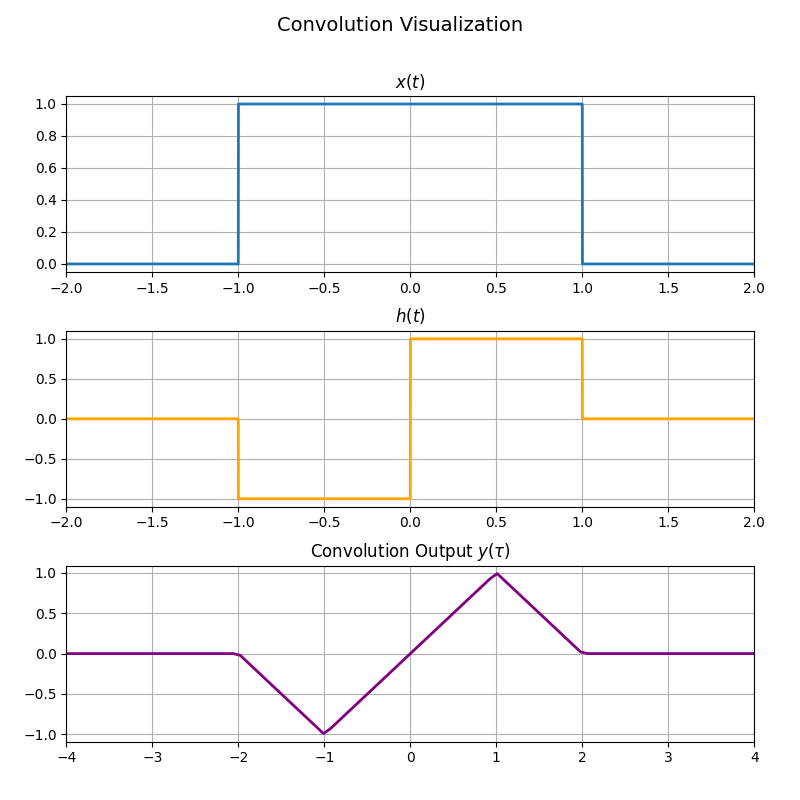
\includegraphics[width=0.8\textwidth]{images/problem_2_1_snapshot.png}
\end{center}
\end{tosubmit}
% ==================== %

\newpage 

% === Problem 2.3. === %
\begin{tosubmit}
\begin{subproblems}[start=3]
    \item \submitsolution
\end{subproblems}

Using Python to visualize and compute the convolution graphically,
we can create an animation that demonstrates the convolution process step-by-step
as shown in the gif files in \href{https://github.com/patthadon-p/CEDT-2110203-CEM-II/blob/main/signal/homework-2/images/problem_2_3.gif}{Problem 2.3 Animation}.

\vspace{3mm}

The plot of the signal is shown below:
\begin{center}
    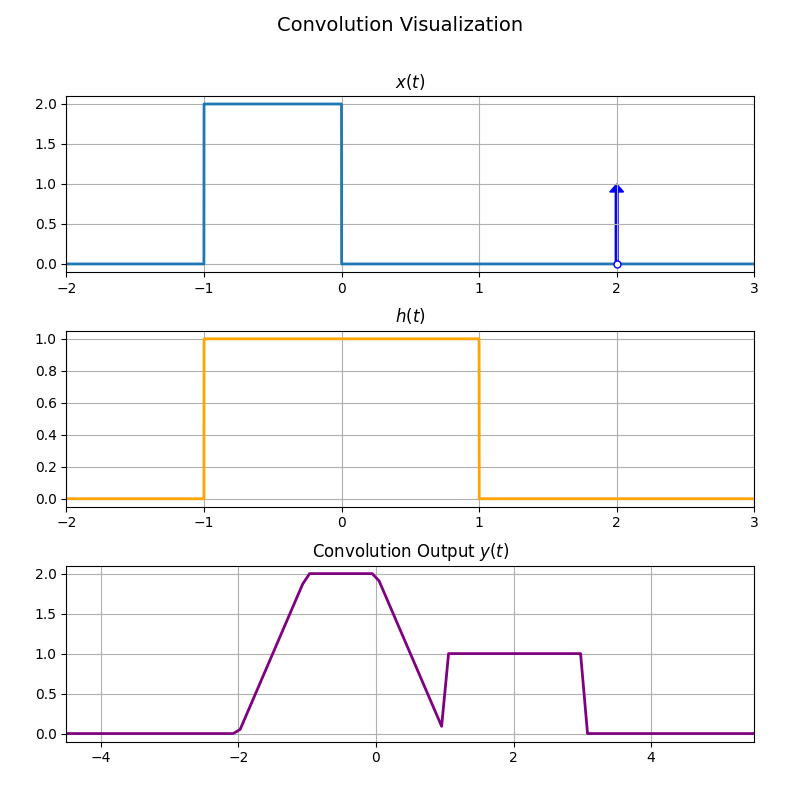
\includegraphics[width=0.8\textwidth]{images/problem_2_3_snapshot.png}
\end{center}
\end{tosubmit}
% ==================== %

\newpage

% ================================================================================ %
%                                    Problem 04                                    %
% ================================================================================ %
\begin{problem}[4]
Find the convolution \( y[n] = h[n] * x[n] \) of the following signals:
\end{problem}

% === Problem 4.1. === %
\begin{tosubmit}
\begin{subproblems}[start=1]
    \item \( x[n] = \begin{cases} -1 , -5 \leq n \leq -1 \\ 1 , 0 \leq n \leq 4 \end{cases},\, h[n] = 2u[n] \)
\end{subproblems}

\par\noindent\submitsolution
Using the property of convolution with unit step function (Running sum):
\[ y[n] = x[n] * u[n] = \sum_{k=-\infty}^{n} x[k] \]

Consider the value of \( y[n] \):
\begin{align*}
    y[n] &= x[n] * h[n] \\
    &= x[n] * 2u[n] \\
    y[n] &= 2 \sum_{k=-\infty}^{n} x[k]
\end{align*}

Calculating the convolution for different ranges of \( n \):
\begin{itemize}
    \item For \( -5 \leq n < 0 \):
    \begin{align*}
        y[n] &= 2 \sum_{k=-\infty}^{n} x[k] \\
        &= 2 \sum_{k=-5}^{n} (-1) \\
        &= 2 \cdot (-1)(n - (-5) + 1) \\
        &= 2 (-n - 6) \\
        y[n] &= -2n - 12
    \end{align*}

    \item For \( 0 \leq n < 5 \):
    \begin{align*}
        y[n] &= 2 \sum_{k=-\infty}^{n} x[k] \\
        &= 2 \sqbracket{ \sum_{k=-5}^{-1} x[k] + \sum_{k=0}^{n} x[k] } \\
        &= 2 \sqbracket{ \sum_{k=-5}^{-1} (-1) + \sum_{k=0}^{n} (1) } \\
        &= 2 \paren{ -5 + (n + 1) } \\
        &= 2 \paren{ n - 4 } \\
        y[n] &= 2n - 8
    \end{align*}
\end{itemize}

Thus, the final result of the convolution is:
\[ \boxed{
y[n] = \begin{cases}
-2n - 12 & -5 \leq n < 0 \\
2n - 8 & 0 \leq n < 5 \\
0 & \text{otherwise}
\end{cases}
} \]
\end{tosubmit}
% ==================== %

\newpage

% === Problem 4.3. === %
\begin{tosubmit}    
\begin{subproblems}[start=3]
    \item \( x[n] = \paren{ \frac{1}{2} }^n u[n],\, h[n] = \delta[n] +\delta[n-1] +  \paren{ \frac{1}{3} }^n u[n] \)
\end{subproblems}

\par\noindent\submitsolution
Using the property of convolution with unit step function (Running sum):
\[ y[n] = x[n] * u[n] = \sum_{k=-\infty}^{n} x[k] \]

and the shifting property of convolution:
\[ x[n] * \delta[n - n_0] = x[n - n_0] \]

Consider the value of \( y[n] \):
\begin{align*}
    y[n] &= x[n] * h[n] \\
    &= x[n] * \sqbracket{ \delta[n] + \delta[n - 1] + \paren{ \frac{1}{3} }^n u[n] } \\
    &= \paren{ x[n] * \delta[n] } + \paren{ x[n] * \delta[n - 1] } + \paren{ x[n] * \paren{ \frac{1}{3} }^n u[n] } \\
    y[n] &= \paren{ \frac{1}{2} }^n u[n] + \paren{ \frac{1}{2} }^{n - 1} u[n - 1] + \sum_{k=-\infty}^{n} \paren{ \frac{1}{2} }^k u[k] \paren{ \frac{1}{3} }^{n - k} u[n - k]
\end{align*}

Calculating the convolution for different ranges of \( n \):
\begin{itemize}
    \item For \( n = 0 \):
    \begin{align*}
        y[n] &= \paren{ \frac{1}{2} }^0 u[0] + \paren{ \frac{1}{2} }^{0 - 1} u[0 - 1] + \sum_{k=-\infty}^{0} \paren{ \frac{1}{2} }^k u[k] \paren{ \frac{1}{3} }^{0 - k} u[0 - k] \\
        &= 1 + 0 + \paren{ \frac{1}{2} }^0 u[0] \paren{ \frac{1}{3} }^{0} u[0] \\
        &= 1 + 0 + 1 \\
        y[n] &= 2
    \end{align*}

    \item For \( n \geq 1 \):
    \begin{align*}
        y[n] &= \paren{ \frac{1}{2} }^n u[n] + \paren{ \frac{1}{2} }^{n - 1} u[n - 1] + \sum_{k=-\infty}^{n} \paren{ \frac{1}{2} }^k u[k] \paren{ \frac{1}{3} }^{n - k} u[n - k] \\
        &= \paren{ \frac{1}{2} }^n + \paren{ \frac{1}{2} }^{n - 1} + \sum_{k=0}^{n} \paren{ \frac{1}{2} }^k \paren{ \frac{1}{3} }^{n - k} \\
        &= 3 \paren{ \frac{1}{2} }^n + \paren{ \frac{1}{3} }^{n} \sqbracket{ \sum_{k=0}^{n} \paren{ \frac{3}{2} }^k } \\
        &= 3 \paren{ \frac{1}{2} }^n + \paren{ \frac{1}{3} }^{n} \cdot (-2)\paren{1 - \paren{ \frac{3}{2} }^{n+1}} \\
        y[n] &= 6 \paren{ \frac{1}{2} }^n - 2 \paren{ \frac{1}{3} }^{n}
    \end{align*}
\end{itemize}

Thus, the final result of the convolution is:
\[ \boxed{
y[n] = \begin{cases}
2 & n = 0 \\
6 \paren{ \frac{1}{2} }^n - 2 \paren{ \frac{1}{3} }^n & n \geq 1 \\
0 & \text{otherwise}
\end{cases}
} \]
\end{tosubmit}
% ==================== %
% ================================================================================ %


\end{document}